% !TEX program = xelatex
% 语言与顺序按 lecture/fourier/fourier_series.tex，并补出其中略去的演算
\documentclass[fontset=windows, chinese, 10pt, xcolor=dvipsnames]{beamer}
% Shared preamble for the chapter 04 standalone lectures.
% Each lecture sets \title and \subtitle after this file is read.

\usepackage{amsmath,amssymb,mathtools}
\usepackage{xeCJK}
\usepackage{zhnumber}
\usepackage{tikz}
\usetikzlibrary{arrows.meta,calc,positioning}

\usetheme{metropolis}
\usepackage{beamercolorthemeHistNanjing}

\newcommand{\red}[1]{\textcolor{red}{#1}}
\newcommand{\blue}[1]{\textcolor{blue}{#1}}
\newcommand{\green}[1]{\textcolor{green}{#1}}
\newcommand{\gray}[1]{\textcolor{gray}{#1}}
\newcommand{\orange}[1]{\textcolor{orange}{#1}}

\newcommand{\sssub}[1]{ {\mathrm{#1} }}  % script size subscript\\\
\newcommand{\funcd}[2]{ \frac{d{#1}}{d{#2}}} %function full derivative
\newcommand{\funcpd}[2]{ \frac{\partial{#1}}{\partial{#2}}} %function partial derivative
\newcommand{\fnald}[2] { \frac{\delta {#1}}{\delta {#2}}} % functional derivative

\renewcommand{\Re}{\operatorname{Re}}
\renewcommand{\Im}{\operatorname{Im}}
\def\ext{\sssub{ext}}
\def\x{\sssub{x}}
\def\xc{\sssub{xc}}
\def\H{\sssub{H}}
\def\Hx{\sssub{Hx}}
\def\Hxc{\sssub{Hxc}}
\def\c{\sssub{c}}
\def\s{\sssub{s}}

% \def\ext{\sssub{ext}}
% \def\ext{\sssub{ext}}
% \def\ext{\sssub{ext}}
% \def\ext{\sssub{ext}}
% \defsssub{ext}


% definitions of bold faced symbols
\def\brpppp{{\mathbf{r}^{\prime\prime\prime\prime}}}
\def\brppp{{\mathbf{r}^{\prime\prime\prime}}}
\def\brpp{{\mathbf{r}^{\prime\prime}}}
\def\brp{{\mathbf{r}^{\prime}}}
\def\bzp{{\mathbf{z}^{\prime}}}
\def\bxp{{\mathbf{x}^{\prime}}}
\def\tp{{{t}^{\prime}}}
\def\tpp{{{t}^{\prime\prime}}}
\def\tppp{{{t}^{\prime\prime\prime}}}

\def\tbr{{\tilde{\mathbf{r}}}}
\def\bk{{\mathbf{k}}}
\def\br{{\mathbf{r}}}
\def\bp{{\mathbf{p}}}
\def\bq{{\mathbf{q}}}
\def\bv{{\mathbf{v}}}
\def\bz{{\mathbf{z}}}
\def\mbf{{\mathbf{f}}}

\def\bx{{\mathbf{x}}}
\def\bR{{\mathbf{R}}}
\def\bM{{\mathbf{M}}}
\def\bP{{\mathbf{P}}}
\def\bT{{\mathbf{T}}}
\def\bK{{\mathbf{K}}}
\def\bA{{\mathbf{A}}}
\def\bB{{\mathbf{B}}}
\def\bD{{\mathbf{D}}}
\def\bE{{\mathbf{E}}}
\def\bF{{\mathbf{F}}}
\def\bG{{\mathbf{G}}}
\def\bH{{\mathbf{H}}}
\def\bI{{\mathbf{I}}}
\def\bJ{{\mathbf{J}}}
\def\bP{{\mathbf{P}}}
\def\bS{{\mathbf{S}}}
\def\bV{{\mathbf{V}}}
\def\bX{{\mathbf{X}}}
\def\bY{{\mathbf{Y}}}
\def\dd{{\mathop{}\!\mathrm{d}}}
\def\dr{{\!\!\dd\br\,}}
\def\dx{{\!\!\dd\bx\,}}
\def\dy{{\!\!\dd\by\,}}
\def\dk{{\!\!\dd\bk\,}}
\def\dG{{\!\!\dd\bG\,}}


\def\half{{\frac{1}{2}}}
\def\tr{{\mathrm{tr}}}


\def\Arg{{\mathrm{Arg}\;}}
\def\arg{{\mathrm{arg}\;}}
\def\Res{{\mathrm{Res}\;}}


\author{罗凯}
\institute{南京理工大学物理学院}
\date{\zhdigits{\the\year},\zhganzhinian{\the\year}年秋}

\usebackgroundtemplate{%
\begin{tikzpicture}[remember picture,overlay]
  \node[opacity=0.05, at=(current page.center)] {
    
\includegraphics[width=0.6\paperwidth]{njust-logo.jpeg}
  };
\end{tikzpicture}}

\usepackage{pgfplots}
\pgfplotsset{compat=1.18}

\title{傅里叶分析}
\subtitle{第一讲：傅里叶级数}

\begin{document}

\begin{frame}
  \titlepage
\end{frame}

\begin{frame}{本讲提纲}
  \begin{enumerate}
    \item 正交函数组：内积、施密特正交化、展开系数、贝塞尔不等式与完备性；
    \item 傅里叶级数的引入：均匀棒的热传播、分离变量、正弦叠加；
    \item 傅里叶定理：周期展开、狄里希利条件、有限区间上的延拓、复指数，以及锯齿函数；
    \item 能量定理：Parseval 等式，矩形波给出 $\pi^2/8$。
  \end{enumerate}
\end{frame}

% =============================================================
\section{正交函数组}

\begin{frame}{内积}
  设 $f(x),\,g(x)$ 为定义在区间 $[a,b]$ 上的函数，积分
  \begin{equation*}
    (f,g)\equiv\int_a^b f(x)\,g(x)\,\mathrm{d}x
  \end{equation*}
  叫做二函数 $f(x)$ 和 $g(x)$ 的\textbf{内积} $(f,g)$。
  \vspace{0.5em}

  内积满足\textbf{施瓦茨不等式}
  \begin{equation*}
    |(f,g)|^2\leq (f,f)\,(g,g),
  \end{equation*}
  当且仅当 $f(x)$ 和 $g(x)$ 线性相关时，等号成立。
\end{frame}

\begin{frame}{正交、范数、正交归一组}
  如果 $(f,g)=0$，则称 $f(x)$ 和 $g(x)$ 是\textbf{正交}的。
  函数 $f(x)$ 和它自己的内积称为\textbf{范数}或\textbf{模}，记作 $Nf$，
  \begin{equation*}
    Nf\equiv(f,f)=\int f(x)^2\,\mathrm{d}x.
  \end{equation*}
  范数为 $1$ 的函数称为\textbf{单位函数}或\textbf{归一化函数}。
  \vspace{0.4em}

  一组归一化函数 $\varphi_1,\varphi_2,\cdots$，其中任意二者皆正交，称\textbf{正交归一组}，
  \begin{equation*}
    (\varphi_i,\varphi_j)=\delta_{ij}.
  \end{equation*}
\end{frame}

\begin{frame}{复变函数的内积}
  对于复变函数，内积定义为
  \begin{equation*}
    (f,g)=\int f^*(x)\,g(x)\,\mathrm{d}x,
  \end{equation*}
  其中 $f^*$ 为 $f$ 的复共轭。
  若
  \begin{equation*}
    Nf=\int |f|^2\,\mathrm{d}x=1,
  \end{equation*}
  称函数 $f(x)$ 是归一化的。
\end{frame}

\begin{frame}{正余弦的正交性}
  记 $(f,g)=\displaystyle\int_0^{2\pi} f^*(x)\,g(x)\,\mathrm{d}x$。可以验证，$m,n\neq 0$ 时
  \begin{align*}
    (\sin nx,\sin mx)
      &=(\cos nx,\cos mx)=\pi\,\delta_{mn},\\
    (\sin nx,\cos mx)&=0.
  \end{align*}
  用积化和差。$\sin A\sin B=\tfrac12\bigl[\cos(A-B)-\cos(A+B)\bigr]$。
  $m\neq n$ 时，积分是整周期余弦，结果为零。
  $m=n$ 时
  \begin{equation*}
    \int_0^{2\pi}\tfrac12\bigl(1-\cos 2nx\bigr)\,\mathrm{d}x=\pi.
  \end{equation*}
  余弦与余弦同样。正弦与余弦的积是奇函数在整周期上的积分，为零。
\end{frame}

\begin{frame}{线性相关}
  若对于所有 $x$ 都成立的常系数齐次线性关系
  \begin{equation*}
    \sum_{i=1}^n c_i\,\varphi_i(x)=0
  \end{equation*}
  中系数不全为零，称这 $n$ 个函数\textbf{线性相关}。否则称为\textbf{线性无关}。
  \vspace{0.5em}

  正交组中的各函数永远是线性无关的。
  若上式成立，左乘 $\varphi_j(x)$ 并积分，正交性给出
  \begin{equation*}
    c_j\,(\varphi_j,\varphi_j)=0,
  \end{equation*}
  因而 $c_j=0$。
\end{frame}

\begin{frame}{施密特正交化}
  类比于线性代数中向量的\textbf{施密特正交化}。
  设 $f_1,\ldots,f_n$ 线性无关，令
  \begin{align*}
    \varphi_1&=f_1,\\
    \varphi_k&=f_k-\sum_{j=1}^{k-1}
      \frac{(f_k,\varphi_j)}{(\varphi_j,\varphi_j)}\,\varphi_j.
  \end{align*}
  减号后面是 $f_k$ 在已经造好的 $\varphi_j$ 上的投影。
  再除以各自的范数，就得到正交归一组。
\end{frame}

\begin{frame}{例：$\{1,x\}$ 在 $[0,1]$ 上}
  取 $f_1=1$，$f_2=x$。
  \begin{equation*}
    \varphi_1=1,
    \qquad
    (1,1)=\int_0^1 1\,\mathrm{d}x=1,
    \qquad
    (x,1)=\int_0^1 x\,\mathrm{d}x=\tfrac12.
  \end{equation*}
  于是
  \begin{equation*}
    \varphi_2=x-\frac{(x,\varphi_1)}{(\varphi_1,\varphi_1)}\,\varphi_1
            =x-\tfrac12.
  \end{equation*}
  检验正交：
  \begin{equation*}
    \int_0^1\bigl(x-\tfrac12\bigr)\,\mathrm{d}x
    =\Bigl[\tfrac12 x^2-\tfrac12 x\Bigr]_0^1=0.
  \end{equation*}
\end{frame}

\begin{frame}{展开系数}
  设 $\varphi_1,\ldots,\varphi_n$ 是正交归一组，定义
  \begin{equation*}
    f(x)=\sum_{i=1}^n c_i\,\varphi_i(x),
  \end{equation*}
  其中
  \begin{equation*}
    c_i=(f,\varphi_i)=\int f(x)\,\varphi_i(x)\,\mathrm{d}x
  \end{equation*}
  称为\textbf{展开系数}或\textbf{分量}。
  上式两边乘 $\varphi_j$ 再积分，正交归一只留下 $i=j$ 的一项，就是 $c_j$。
\end{frame}

\begin{frame}{贝塞尔不等式：展开平方}
  由
  \begin{equation*}
    \int\Bigl(f-\sum_{i=1}^n c_i\varphi_i\Bigr)^2\mathrm{d}x\geq 0
  \end{equation*}
  展开平方：
  \begin{equation*}
    \int f^2\,\mathrm{d}x
    -2\sum_{i=1}^n c_i\int f\,\varphi_i\,\mathrm{d}x
    +\sum_{i,j} c_i c_j\int \varphi_i\varphi_j\,\mathrm{d}x\geq 0.
  \end{equation*}
  正交归一使最后一项只剩 $\sum c_i^2$，中间一项的积分就是 $c_i$，所以
  \begin{equation*}
    Nf-2\sum_{i=1}^n c_i^2+\sum_{i=1}^n c_i^2\geq 0,
  \end{equation*}
  即
  \begin{equation*}
    \sum_{i=1}^n c_i^2\leq Nf.
  \end{equation*}
\end{frame}

\begin{frame}{贝塞尔不等式}
  上式可以令 $n\to\infty$，得到
  \begin{equation*}
    \sum_{i=1}^{\infty} c_i^2\leq Nf.
  \end{equation*}
  这称为\textbf{贝塞尔不等式}。它对每一个正交归一组都成立，它证明了展开系数的平方和是收敛有界的。
\end{frame}

\begin{frame}{完备}
  假如有一正交归一组，使得对任意分段连续函数 $f(x)$，都有 $n$ 使\textbf{平均平方误差}
  \begin{equation*}
    \int\Bigl(f(x)-\sum_{i=1}^n c_i\varphi_i(x)\Bigr)^2\mathrm{d}x
  \end{equation*}
  小于任意给定正数 $\epsilon$，那么称 $\varphi_1,\varphi_2,\cdots$ 是\textbf{完备}的。
  \vspace{0.4em}

  对于完备的正交归一组，贝塞尔不等式对任意函数都成为等式
  \begin{equation*}
    \sum_{i=1}^{\infty} c_i^2=Nf,
  \end{equation*}
  这个关系称为\textbf{完备性关系}。三角函数族满足这一关系。
\end{frame}

% =============================================================
\section{傅里叶级数的引入}

\begin{frame}{均匀棒的热传播}
  Fourier 曾试图解决一个问题，在此过程中发展了傅里叶级数的概念。
  此问题处理长度为 $\ell$ 的一维均匀棒的热传播：给定初始温度分布，求解 $t$ 时刻、$x$ 处的温度 $T(x,t)$。该温度场满足
  \begin{equation*}
    \frac{\partial^2 T}{\partial x^2}
      =\frac{\partial T}{\partial t},
    \qquad
    T(0,t)=T(\ell,t)=0.
  \end{equation*}
\end{frame}

\begin{frame}{分离变量}
  该方程的一特殊解可以由\textbf{分离变量法}得到。令 $T(x,t)=f(x)\,g(t)$，代入得
  \begin{equation*}
    f''(x)\,g(t)=f(x)\,g'(t).
  \end{equation*}
  两边同除以 $f(x)g(t)$，
  \begin{equation*}
    \frac{f''(x)}{f(x)}=\frac{g'(t)}{g(t)}.
  \end{equation*}
  左式与 $t$ 无关，右边与 $x$ 无关，于是二者皆为同一个常数 $c$。
\end{frame}

\begin{frame}{常数取 $-k^2$}
  这时候若 $c>0$，记 $c=\kappa^2$，则 $g'(t)=\kappa^2 g(t)$，
  \begin{equation*}
    g(t)=C\,e^{\kappa^2 t},
    \qquad
    \lim_{t\to\infty} g(t)=\infty.
  \end{equation*}
  温度不会随时间无限升高，因此令 $c=-k^2$。两个常微分方程是
  \begin{equation*}
    f''+k^2 f=0,
    \qquad
    g'+k^2 g=0.
  \end{equation*}
  通解
  \begin{equation*}
    f(x)=A\sin(kx)+B\cos(kx),
    \qquad
    g(t)=e^{-k^2 t}.
  \end{equation*}
\end{frame}

\begin{frame}{边界条件定出 $k$}
  $T(0,t)=f(0)g(t)=0$。$g(t)$ 不恒为零，所以 $f(0)=B=0$。
  \vspace{0.3em}

  $T(\ell,t)=0$ 要求 $\sin(k\ell)=0$，故
  \begin{equation*}
    k\ell=n\pi,
    \qquad
    k=\frac{n\pi}{\ell},
    \qquad n=1,2,\ldots.
  \end{equation*}
  一个模式是
  \begin{equation*}
    T(x,t)
    =A\sin\Bigl(\frac{n\pi}{\ell}x\Bigr)
     e^{-n^2\pi^2 t/\ell^2}.
  \end{equation*}
  $t=0$ 时，$T$ 为一个正弦函数，节点数由 $n$ 决定。
\end{frame}

\begin{frame}{线性叠加}
  更普遍的情况是起始时刻的温度分布并不是正弦函数。
  对于线性微分方程，若 $T_1$、$T_2$ 都满足方程，则任意线性组合
  \begin{equation*}
    T_3=\alpha T_1+\beta T_2
  \end{equation*}
  也是解。两端为零的边界条件同样被保持。
  \vspace{0.4em}

  对于任意一种光滑的温度分布，其解总可以写成一系列有着不同振幅和模式的正弦函数的线性叠加：
  \begin{equation*}
    T(x,t)=\sum_{n=1}^{\infty}
      A_n\sin\Bigl(\frac{n\pi}{\ell}x\Bigr)
      e^{-n^2\pi^2 t/\ell^2}.
  \end{equation*}
\end{frame}

\begin{frame}{初始温度}
  若初始温度分布为 $f(x)=T(x,0)$，指数因子在 $t=0$ 时等于 $1$，于是
  \begin{equation*}
    f(x)=\sum_{n=1}^{\infty}
      A_n\sin\Bigl(\frac{n\pi}{\ell}x\Bigr).
  \end{equation*}
  什么样的函数可以表示为正弦和余弦函数的叠加？每个模式的振幅 $A_n$ 该如何计算？这就利用了正余弦函数的特征。
\end{frame}

\begin{frame}{改到区间 $[0,\ell]$}
  前面的正交性写在 $[0,2\pi]$ 上。热棒的区间是 $[0,\ell]$。令
  \begin{equation*}
    \theta=\frac{\pi x}{\ell},
    \qquad
    \mathrm{d}x=\frac{\ell}{\pi}\,\mathrm{d}\theta,
  \end{equation*}
  $x$ 从 $0$ 到 $\ell$ 时，$\theta$ 从 $0$ 到 $\pi$。于是
  \begin{align*}
    \int_0^{\ell}
      \sin\Bigl(\frac{n\pi x}{\ell}\Bigr)
      \sin\Bigl(\frac{m\pi x}{\ell}\Bigr)
      \,\mathrm{d}x
    &=\frac{\ell}{\pi}\int_0^{\pi}\sin(n\theta)\sin(m\theta)\,\mathrm{d}\theta \\
    &=\frac{\ell}{2}\,\delta_{mn}.
  \end{align*}
  这里用了半周期上的正交性：正整数 $n,m$ 满足
  $\displaystyle\int_0^{\pi}\sin(n\theta)\sin(m\theta)\,\mathrm{d}\theta=\tfrac{\pi}{2}\delta_{mn}$。
\end{frame}

\begin{frame}{半周期上仍正交}
  正整数 $n,m$ 在 $[0,\pi]$ 上仍正交。积化和差
  \begin{equation*}
    \sin(n\theta)\sin(m\theta)
    =\frac12\Bigl[
      \cos\bigl((n-m)\theta\bigr)
      -\cos\bigl((n+m)\theta\bigr)
    \Bigr].
  \end{equation*}
  $n\neq m$ 时，$n-m$ 与 $n+m$ 都是非零整数，
  \begin{equation*}
    \int_0^{\pi}\cos(k\theta)\,\mathrm{d}\theta
    =\frac{\sin(k\pi)}{k}=0.
  \end{equation*}
  $n=m$ 时
  \begin{equation*}
    \int_0^{\pi}\frac12\bigl(1-\cos(2n\theta)\bigr)\,\mathrm{d}\theta
    =\frac{\pi}{2}.
  \end{equation*}
  因此 $\displaystyle\int_0^{\pi}\sin(n\theta)\sin(m\theta)\,\mathrm{d}\theta=\tfrac{\pi}{2}\delta_{mn}$，
  热棒上的范数是 $\ell/2$。
\end{frame}

\begin{frame}{振幅系数}
  用 $\sin(m\pi x/\ell)$ 乘初始温度的展开，再从 $0$ 积到 $\ell$。左边
  \begin{equation*}
    \int_0^{\ell} f(x)\sin\Bigl(\frac{m\pi x}{\ell}\Bigr)\,\mathrm{d}x.
  \end{equation*}
  右边只有 $n=m$ 的一项留下来，系数是 $A_m\cdot\ell/2$。因此
  \begin{equation*}
    A_n=\frac{2}{\ell}\int_0^{\ell}
      f(x)\sin\Bigl(\frac{n\pi}{\ell}x\Bigr)\,\mathrm{d}x.
  \end{equation*}
  $A_n$ 称为傅里叶级数的\textbf{系数}。若所有系数都求得后，我们就得到了 $f(x)$。自然，越多的级数项对函数的逼近也就越好。
\end{frame}

% =============================================================
\section{傅里叶定理}

\begin{frame}{以 $2\ell$ 为周期}
  对于任意一个以 $2\ell$ 为周期的函数，$f(x+2\ell)=f(x)$，可以通过三角函数族进行级数展开
  \begin{equation*}
    f(x)=\frac{a_0}{2}+\sum_{n=1}^{\infty}
      \Bigl[
        a_n\cos\frac{n\pi x}{\ell}
        +b_n\sin\frac{n\pi x}{\ell}
      \Bigr].
  \end{equation*}
  利用三角函数族的正交性，在一个周期上
  \begin{align*}
    \int_{-\ell}^{\ell}
      \cos\frac{n\pi x}{\ell}
      \cos\frac{m\pi x}{\ell}\,\mathrm{d}x
      &=\ell\,\delta_{mn}
      \quad(n,m\geq 1),\\
    \int_{-\ell}^{\ell} 1\,\mathrm{d}x&=2\ell,
  \end{align*}
  正弦与正弦同样得到 $\ell\,\delta_{mn}$，正弦与余弦的积分为零。
\end{frame}

\begin{frame}{系数公式}
  展开式乘 $\cos(m\pi x/\ell)$，从 $-\ell$ 积到 $\ell$。
  $m\geq 1$ 时只留下 $a_m\cdot\ell$，所以
  \begin{equation*}
    a_n=\frac{1}{\ell}\int_{-\ell}^{\ell}
      f(x)\cos\Bigl(\frac{n\pi}{\ell}x\Bigr)\,\mathrm{d}x.
  \end{equation*}
  常数项：$a_0/2$ 乘上区间长度 $2\ell$，等于 $\displaystyle\int_{-\ell}^{\ell} f\,\mathrm{d}x$，因此 $n=0$ 仍用同一个公式。
  \vspace{0.3em}

  乘 $\sin(m\pi x/\ell)$ 则得到
  \begin{equation*}
    b_n=\frac{1}{\ell}\int_{-\ell}^{\ell}
      f(x)\sin\Bigl(\frac{n\pi}{\ell}x\Bigr)\,\mathrm{d}x.
  \end{equation*}
  积分上下限为一个周期 $2\ell$，也可以取 $[0,2\ell]$。
\end{frame}

\begin{frame}{狄里希利条件}
  上述展开的成立条件被称为\textbf{狄里希利条件}：
  $f(x)$ 在 $[-\ell,\ell]$ 内只有有限个间断点，且每个周期内有有限个极值点。
  满足这两个条件的函数称为\textbf{分段平常}。
  \vspace{0.5em}

  满足狄里希利条件的函数在点 $x_0$ 处间断，那么其傅里叶级数在此点的值为该函数左右值的算术平均
  \begin{equation*}
    \lim_{\epsilon\to 0}\frac12
      \bigl[f(x_0+\epsilon)+f(x_0-\epsilon)\bigr].
  \end{equation*}
\end{frame}

\begin{frame}{分段平常的例子}
  一个周期内只有有限个间断点，也只有有限个极值点。空心点表示该点不取曲线上的值。
  \vspace{0.7em}
  \begin{columns}[t]
    \begin{column}{0.33\textwidth}
      \centering
      \begin{tikzpicture}[x=0.38cm,y=0.62cm,>=Stealth]
        \draw[->] (-3.7,0) -- (3.9,0) node[right] {$x$};
        \draw[->] (0,-1.8) -- (0,2.15) node[above] {$f$};
        \draw[thick] (-3.14,-1) -- (-0.12,-1);
        \draw[thick] (0.12,1) -- (3.14,1);
        \draw[fill=white] (-3.14,-1) circle (1.5pt);
        \draw[fill=white] (0,-1) circle (1.5pt);
        \draw[fill=white] (0,1) circle (1.5pt);
        \draw[fill=white] (3.14,1) circle (1.5pt);
        \node[below] at (-3.14,0) {$-\pi$};
        \node[below] at (3.14,0) {$\pi$};
        \node[left] at (0,1) {$1$};
        \node[left] at (0,-1) {$-1$};
      \end{tikzpicture}\\[0.45em]
      {\small 矩形波：两个跳跃}
    \end{column}
    \begin{column}{0.33\textwidth}
      \centering
      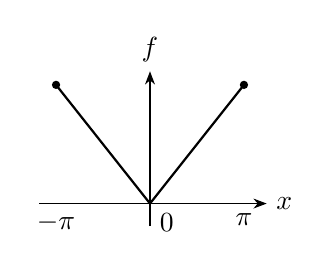
\begin{tikzpicture}[x=0.38cm,y=0.48cm,>=Stealth]
        \draw[->] (-3.7,0) -- (3.9,0) node[right] {$x$};
        \draw[->] (0,-0.6) -- (0,3.5) node[above] {$f$};
        \draw[thick] (-3.14,3.14) -- (0,0) -- (3.14,3.14);
        \fill (-3.14,3.14) circle (1.5pt);
        \fill (3.14,3.14) circle (1.5pt);
        \node[below] at (-3.14,0) {$-\pi$};
        \node[below] at (3.14,0) {$\pi$};
        \node[below right] at (0,0) {$0$};
      \end{tikzpicture}\\[0.45em]
      {\small 绝对值：连续，一个极小}
    \end{column}
    \begin{column}{0.33\textwidth}
      \centering
      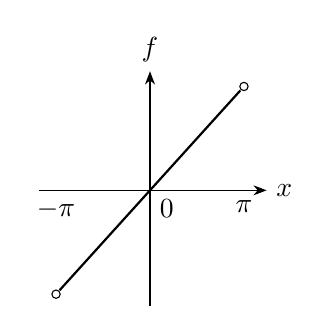
\begin{tikzpicture}[x=0.38cm,y=0.42cm,>=Stealth]
        \draw[->] (-3.7,0) -- (3.9,0) node[right] {$x$};
        \draw[->] (0,-3.5) -- (0,3.6) node[above] {$f$};
        \draw[thick] (-3.02,-3.02) -- (3.02,3.02);
        \draw[fill=white] (-3.14,-3.14) circle (1.5pt);
        \draw[fill=white] (3.14,3.14) circle (1.5pt);
        \node[below] at (-3.14,0) {$-\pi$};
        \node[below] at (3.14,0) {$\pi$};
        \node[below right] at (0,0) {$0$};
      \end{tikzpicture}\\[0.45em]
      {\small 锯齿 $f(x)=x$：端点一个跳跃}
    \end{column}
  \end{columns}
\end{frame}

\begin{frame}{正弦级数与余弦级数}
  对于奇函数和偶函数，不难发现：奇函数的 $a_n$ 全为零，展开为
  \begin{equation*}
    f(x)=\sum_{n=1}^{\infty}
      b_n\sin\Bigl(\frac{n\pi}{\ell}x\Bigr),
  \end{equation*}
  称为\textbf{傅里叶正弦级数}。
  偶函数的 $b_n$ 全为零，展开为
  \begin{equation*}
    f(x)=\frac{a_0}{2}+\sum_{n=1}^{\infty}
      a_n\cos\Bigl(\frac{n\pi}{\ell}x\Bigr),
  \end{equation*}
  称为\textbf{傅里叶余弦级数}。
  热棒两端为零，初始温度奇延拓到 $[-\ell,\ell]$ 后是奇函数，所以只出现正弦。
\end{frame}

\begin{frame}{有限区间上的函数}
  对于只在有限区间，例如在 $(0,\ell)$ 上有定义的函数 $f(x)$，可以采取\textbf{延拓}的方法，使其成为某种周期函数 $g(x)$，而在 $(0,\ell)$ 上，$g(x)\equiv f(x)$。然后再对 $g(x)$ 作傅里叶展开，其级数和在区间 $(0,\ell)$ 上代表 $f(x)$。
  \vspace{0.5em}

  由于 $f(x)$ 在 $(0,\ell)$ 以外无定义，因此可以有无数种延拓方式，从而有无数种展开式，但它们在 $(0,\ell)$ 上均代表 $f(x)$。
\end{frame}

\begin{frame}{边界条件决定延拓}
  有时，对函数 $f(x)$ 在边界（区间的端点）上的行为提出限制，即满足一定的边界条件，这常常就决定了如何延拓。
  \vspace{0.4em}

  例如要求 $f(0)=f(\ell)=0$，这时应延拓成为\textbf{奇的周期函数}。
  又如要求 $f'(0)=f'(\ell)=0$，这时则应延拓成\textbf{偶的周期函数}。
\end{frame}

\begin{frame}{奇延拓}
  把 $f$ 延拓成以 $2\ell$ 为周期的奇函数：在 $(0,\ell)$ 上 $g=f$，
  \begin{equation*}
    g(-x)=-g(x),
    \qquad
    g(x+2\ell)=g(x).
  \end{equation*}
  于是 $-\ell<x<0$ 时 $g(x)=-f(-x)$。奇函数的余弦系数为零，
  \begin{equation*}
    f(x)=\sum_{n=1}^{\infty} b_n\sin\frac{n\pi x}{\ell},
    \quad
    b_n=\frac{2}{\ell}\int_0^{\ell} f(x)\sin\frac{n\pi x}{\ell}\,\mathrm{d}x.
  \end{equation*}
\end{frame}

% \begin{frame}{为什么是 $f(0)=f(\ell)=0$}
%   由周期性，$g(\ell+\epsilon)=g(-\ell+\epsilon)$。再由奇性，$g(-\ell+\epsilon)=-g(\ell-\epsilon)$。因此
%   \begin{equation*}
%     g(\ell+\epsilon)=-g(\ell-\epsilon).
%   \end{equation*}
%   $g$ 关于 $x=\ell$ 也是奇的。连续延拓时左右极限相等，只能是
%   \begin{equation*}
%     g(0)=0,
%     \qquad
%     g(\ell)=0.
%   \end{equation*}
%   正弦级数在端点自动为零，与 $f(0)=f(\ell)=0$ 一致。热棒两端保持零度，用的就是这个延拓。
% \end{frame}

\begin{frame}{偶延拓}
  要求 $f'(0)=f'(\ell)=0$ 时，延拓成以 $2\ell$ 为周期的偶函数：
  \begin{equation*}
    g(-x)=g(x),
    \qquad
    -\ell<x<0 \text{ 时 } g(x)=f(-x).
  \end{equation*}
  偶函数的正弦系数为零，
  \begin{equation*}
    f(x)=\frac{a_0}{2}+\sum_{n=1}^{\infty} a_n\cos\frac{n\pi x}{\ell},
    \quad
    a_n=\frac{2}{\ell}\int_0^{\ell} f(x)\cos\frac{n\pi x}{\ell}\,\mathrm{d}x.
  \end{equation*}
\end{frame}

\begin{frame}{延拓的图例}
  取 $(0,\ell)$ 上的 $f(x)=x$。\blue{蓝线}是给定的一段，\orange{橙线}是延拓，周期为 $2\ell$。空心点表示跳跃处不取曲线上的值。
  \vspace{0.55em}
  \begin{columns}[t]
    \begin{column}{0.5\textwidth}
      \centering
      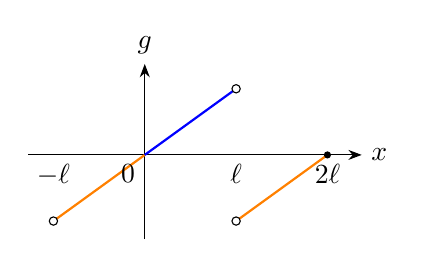
\begin{tikzpicture}[x=0.58cm,y=0.42cm,>=Stealth]
        \draw[->] (-2.55,0) -- (4.75,0) node[right] {$x$};
        \draw[->] (0,-2.55) -- (0,2.75) node[above] {$g$};
        \draw[orange,thick] (-2,-2) -- (0,0);
        \draw[blue,thick] (0,0) -- (2,2);
        \draw[orange,thick] (2,-2) -- (4,0);
        \draw[fill=white] (-2,-2) circle (1.5pt);
        \draw[fill=white] (2,2) circle (1.5pt);
        \draw[fill=white] (2,-2) circle (1.5pt);
        \fill (4,0) circle (1.3pt);
        \node[below] at (-2,0) {$-\ell$};
        \node[below] at (2,0) {$\ell$};
        \node[below] at (4,0) {$2\ell$};
        \node[below left] at (0,0) {$0$};
      \end{tikzpicture}\\[0.4em]
      {\small 奇延拓：$g(-x)=-g(x)$，正弦级数\\
      在 $x=\ell$ 处跳跃}
    \end{column}
    \begin{column}{0.5\textwidth}
      \centering
      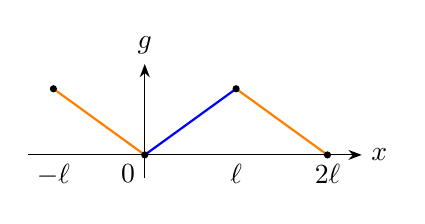
\begin{tikzpicture}[x=0.58cm,y=0.42cm,>=Stealth]
        \draw[->] (-2.55,0) -- (4.75,0) node[right] {$x$};
        \draw[->] (0,-0.7) -- (0,2.75) node[above] {$g$};
        \draw[orange,thick] (-2,2) -- (0,0);
        \draw[blue,thick] (0,0) -- (2,2);
        \draw[orange,thick] (2,2) -- (4,0);
        \fill (-2,2) circle (1.3pt);
        \fill (0,0) circle (1.3pt);
        \fill (2,2) circle (1.3pt);
        \fill (4,0) circle (1.3pt);
        \node[below] at (-2,0) {$-\ell$};
        \node[below] at (2,0) {$\ell$};
        \node[below] at (4,0) {$2\ell$};
        \node[below left] at (0,0) {$0$};
      \end{tikzpicture}\\[0.4em]
      {\small 偶延拓：$g(-x)=g(x)$，余弦级数\\
      在 $x=0,\ell$ 处连续}
    \end{column}
  \end{columns}
\end{frame}

% \begin{frame}{为什么是 $f'(0)=f'(\ell)=0$}
%   偶函数的导数是奇函数。$x>0$ 时 $g'(x)=f'(x)$；$x<0$ 时
%   \begin{equation*}
%     g'(x)=\frac{\mathrm{d}}{\mathrm{d}x}f(-x)=-f'(-x).
%   \end{equation*}
%   左右导数在 $x=0$ 处相等，当且仅当 $f'(0)=0$，此时 $g'(0)=0$。
%   \vspace{0.4em}
%
%   与奇延拓同样的移轴可知，$g$ 关于 $x=\ell$ 是偶的，导数关于 $x=\ell$ 是奇的。导数在 $x=\ell$ 处存在，就要求 $f'(\ell)=0$。余弦级数的导数是正弦级数，在 $x=0$ 和 $x=\ell$ 自动为零。
% \end{frame}

\begin{frame}{复指数形式}
  由欧拉公式
  \begin{equation*}
    \cos\theta=\frac{e^{\mathrm{i}\theta}+e^{-\mathrm{i}\theta}}{2},
    \qquad
    \sin\theta=\frac{e^{\mathrm{i}\theta}-e^{-\mathrm{i}\theta}}{2\mathrm{i}},
  \end{equation*}
  令 $\theta=n\pi x/\ell$。$a_n\cos\theta$ 贡献 $\tfrac12 a_n$ 给 $e^{\mathrm{i}\theta}$ 和 $e^{-\mathrm{i}\theta}$；
  $b_n\sin\theta$ 贡献 $b_n/(2\mathrm{i})=-\mathrm{i}\,b_n/2$ 给 $e^{\mathrm{i}\theta}$，以及 $\mathrm{i}\,b_n/2$ 给 $e^{-\mathrm{i}\theta}$。
  合并后
  \begin{equation*}
    f(x)=\sum_{n=-\infty}^{\infty}
      c_n\,e^{\mathrm{i} n\pi x/\ell},
  \end{equation*}
  其中 $n>0$ 时
  \begin{equation*}
    c_n=\tfrac12(a_n-\mathrm{i} b_n),
    \quad
    c_{-n}=\tfrac12(a_n+\mathrm{i} b_n),
    \quad
    c_0=\tfrac12 a_0.
  \end{equation*}
\end{frame}

\begin{frame}{复系数的积分}
  写出来为
  \begin{equation*}
    c_n=\frac{1}{2\ell}\int_{-\ell}^{\ell}
      f(x)\,e^{-\mathrm{i} n\pi x/\ell}\,\mathrm{d}x.
  \end{equation*}
  尽管 $f(x)$ 是实数，但其傅里叶系数却可能是复数。
  由上式还可以看出 $c_{-n}=c_n^*$。
  \vspace{0.4em}

  复指数函数族也是正交的。$n\neq m$ 时指数的积分是整周期，为零；$n=m$ 时被积函数为 $1$，
  \begin{equation*}
    \int_{-\ell}^{\ell}
      e^{-\mathrm{i} n\pi x/\ell}
      e^{\mathrm{i} m\pi x/\ell}\,\mathrm{d}x
    =2\ell\,\delta_{mn}.
  \end{equation*}
\end{frame}

\begin{frame}{例：锯齿函数}
  \begin{columns}[c]
    \begin{column}{0.52\textwidth}
      \begin{equation*}
        f(x)=\begin{cases}
          x, & 0<x\leq\ell,\\
          x-2\ell, & \ell<x\leq 2\ell.
        \end{cases}
      \end{equation*}
      求其傅里叶级数。它是奇函数，余弦系数为零。
      \vspace{0.35em}

      按 $[0,2\ell]$ 上的正弦公式，$k=n\pi/\ell$，
      \begin{equation*}
        \begin{aligned}
          b_n
          &=\frac{1}{\ell}\int_0^{\ell} x\sin(kx)\,\mathrm{d}x\\
          &\quad+\frac{1}{\ell}\int_{\ell}^{2\ell}(x-2\ell)\sin(kx)\,\mathrm{d}x.
        \end{aligned}
      \end{equation*}
    \end{column}
    \begin{column}{0.46\textwidth}
      \centering
      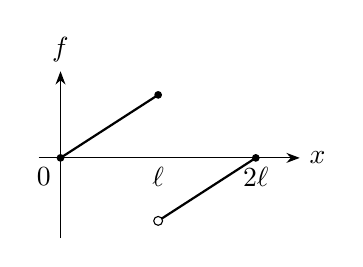
\begin{tikzpicture}[x=0.62cm,y=0.40cm,>=Stealth]
        \draw[->] (-0.45,0) -- (4.9,0) node[right] {$x$};
        \draw[->] (0,-2.55) -- (0,2.75) node[above] {$f$};
        \draw[thick] (0,0) -- (2,2);
        \draw[thick] (2,-2) -- (4,0);
        \fill (0,0) circle (1.4pt);
        \fill (2,2) circle (1.4pt);
        \draw[fill=white] (2,-2) circle (1.6pt);
        \fill (4,0) circle (1.4pt);
        \node[below left] at (0,0) {$0$};
        \node[below] at (2,0) {$\ell$};
        \node[below] at (4,0) {$2\ell$};
      \end{tikzpicture}
    \end{column}
  \end{columns}
\end{frame}

\begin{frame}{锯齿函数：第一段}
  分部积分。令 $u=x$，$\mathrm{d}v=\sin(kx)\,\mathrm{d}x$，则 $\mathrm{d}u=\mathrm{d}x$，$v=-\cos(kx)/k$。
  \begin{align*}
    \int_0^{\ell} x\sin(kx)\,\mathrm{d}x
    &=\Bigl[-\frac{x\cos(kx)}{k}\Bigr]_0^{\ell}
      +\frac{1}{k}\int_0^{\ell}\cos(kx)\,\mathrm{d}x \\
    &=-\frac{\ell\cos(n\pi)}{k}
      +\frac{\sin(n\pi)-\sin 0}{k^2}.
  \end{align*}
  $\sin(n\pi)=0$，$\cos(n\pi)=(-1)^n$，所以
  \begin{equation*}
    \int_0^{\ell} x\sin(kx)\,\mathrm{d}x
    =\frac{\ell}{k}(-1)^{n+1}
    =\frac{\ell^2}{n\pi}(-1)^{n+1}.
  \end{equation*}
\end{frame}

\begin{frame}{锯齿函数：第二段}
  同样分部。令 $u=x-2\ell$，$v=-\cos(kx)/k$。边界项在 $x=2\ell$ 为零；在 $x=\ell$，
  \begin{equation*}
    -\frac{(\ell-2\ell)\cos(n\pi)}{k}
    =\frac{\ell\,(-1)^n}{k}.
  \end{equation*}
  上下限相减，
  \begin{equation*}
    0-\frac{\ell\,(-1)^n}{k}
    =\frac{\ell}{k}(-1)^{n+1}.
  \end{equation*}
  $\displaystyle\int_{\ell}^{2\ell}\cos(kx)\,\mathrm{d}x=\sin(2n\pi)-\sin(n\pi)=0$。
  因此第二段积分与第一段相同，
  \begin{equation*}
    \int_{\ell}^{2\ell}(x-2\ell)\sin(kx)\,\mathrm{d}x
    =\frac{\ell^2}{n\pi}(-1)^{n+1}.
  \end{equation*}
  两段相加再除以 $\ell$，
  \begin{equation*}
    b_n=\frac{2\ell}{n\pi}(-1)^{n+1}.
  \end{equation*}
\end{frame}

\begin{frame}{锯齿函数的级数}
  因此
  \begin{equation*}
    f(x)=\frac{2\ell}{\pi}\sum_{n=1}^{\infty}
      \frac{(-1)^{n+1}}{n}
      \sin\Bigl(\frac{n\pi x}{\ell}\Bigr).
  \end{equation*}
  写开为
  \begin{equation*}
    f(x)=\frac{2\ell}{\pi}\Biggl[
      \sin\frac{\pi x}{\ell}
      -\frac12\sin\frac{2\pi x}{\ell}
      +\frac13\sin\frac{3\pi x}{\ell}-\cdots
    \Biggr].
  \end{equation*}
  其实，这个锯齿函数可以直接用 $f(x)=x$（$-\ell<x<\ell$）来表示，相应的间断点则被移到 $\pm\ell$ 处。奇函数的系数公式 $b_n=(2/\ell)\int_0^{\ell} x\sin(kx)\,\mathrm{d}x$ 给出同一个结果。
\end{frame}

\begin{frame}{部分和逼近锯齿函数}
  前 $N$ 项部分和
  \begin{equation*}
    s_N(x)=\frac{2\ell}{\pi}\sum_{n=1}^{N}
      \frac{(-1)^{n+1}}{n}
      \sin\Bigl(\frac{n\pi x}{\ell}\Bigr).
  \end{equation*}
  $N$ 增大时，$s_N$ 在连续处贴近 $f$，间断点 $x=\ell$ 附近仍有过冲。
  \centering
  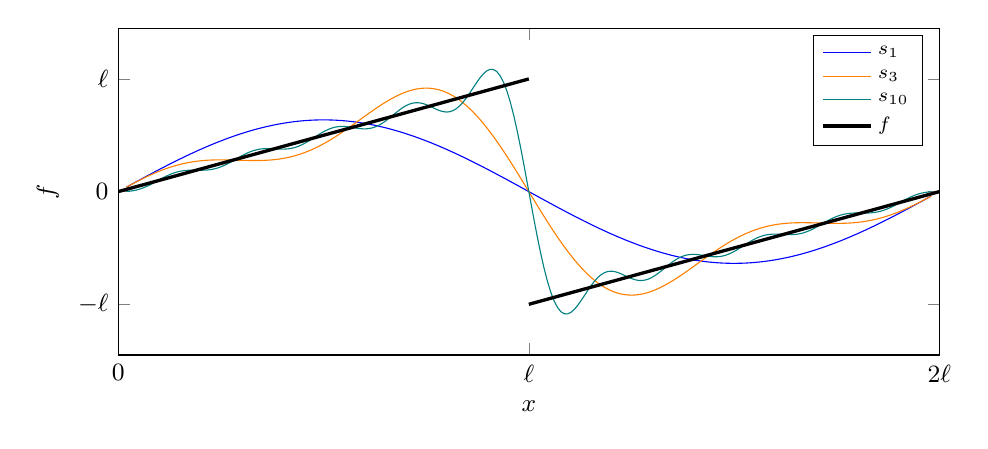
\begin{tikzpicture}
    \begin{axis}[
      width=0.86\textwidth,
      height=4.15cm,
      scale only axis,
      xmin=0, xmax=2,
      ymin=-1.45, ymax=1.45,
      xtick={0,1,2},
      xticklabels={$0$,$\ell$,$2\ell$},
      ytick={-1,0,1},
      yticklabels={$-\ell$,$0$,$\ell$},
      xlabel={$x$},
      ylabel={$f$},
      tick label style={font=\small},
      label style={font=\small},
      legend style={font=\scriptsize, cells={anchor=west}, at={(0.98,0.98)}, anchor=north east},
      every axis plot/.append style={no markers},
      samples=240,
      domain=0.02:1.98,
    ]
      \addplot[blue] {(2/pi)*sin(deg(pi*x))};
      \addlegendentry{$s_1$}
      \addplot[orange] {(2/pi)*(
        sin(deg(pi*x))
        -sin(deg(2*pi*x))/2
        +sin(deg(3*pi*x))/3
      )};
      \addlegendentry{$s_3$}
      \addplot[teal] {(2/pi)*(
        sin(deg(pi*x))
        -sin(deg(2*pi*x))/2
        +sin(deg(3*pi*x))/3
        -sin(deg(4*pi*x))/4
        +sin(deg(5*pi*x))/5
        -sin(deg(6*pi*x))/6
        +sin(deg(7*pi*x))/7
        -sin(deg(8*pi*x))/8
        +sin(deg(9*pi*x))/9
        -sin(deg(10*pi*x))/10
      )};
      \addlegendentry{$s_{10}$}
      \addplot[black, very thick, forget plot, domain=0:1, samples=2] {x};
      \addplot[black, very thick, domain=1:2, samples=2] {x-2};
      \addlegendentry{$f$}
    \end{axis}
  \end{tikzpicture}
\end{frame}

\begin{frame}{Gibbs 现象}
  间断点附近的过冲称为\textbf{Gibbs 现象}。它不是级数和的错误：无穷级数在 $x=\ell$ 仍等于左右极限的算术平均 $0$。过冲出现在部分和 $s_N$ 里。
  \vspace{0.45em}

  跳跃高度是左右极限之差。锯齿函数在 $x=\ell$ 从 $\ell$ 跳到 $-\ell$，高度为 $2\ell$。$N$ 很大时，部分和在跳跃两侧各冲出跳跃高度的固定比例
  \begin{equation*}
    \frac{1}{\pi}\int_0^{\pi}\frac{\sin t}{t}\,\mathrm{d}t-\frac12
    \approx 0.089,
  \end{equation*}
  约 $9\%$。第一峰因此趋于约 $1.18\ell$，而不是 $\ell$。
  \vspace{0.45em}

  $N$ 增大时，这个比例几乎不变，振荡只是挤向间断点，宽度大约按 $1/N$ 缩小。过冲占的区间越来越窄，平均平方误差仍然趋于零。
\end{frame}

\begin{frame}{莱布尼兹等式}
  容易验证：$f(0)=0$。在间断点 $x=\ell$，左极限为 $\ell$，右极限为 $-\ell$，算术平均为 $0$，级数和也是 $0$。
  \vspace{0.4em}

  当 $x=\ell/2$，$f(\ell/2)=\ell/2$。偶数项的正弦为零，$\sin(\pi/2)=1$，$\sin(3\pi/2)=-1$，于是
  \begin{equation*}
    \frac{\ell}{2}
    =\frac{2\ell}{\pi}\Biggl[
      1-\frac13+\frac15-\frac17+\cdots
    \Biggr].
  \end{equation*}
  约去 $\ell$，得到\textbf{莱布尼兹等式}
  \begin{equation*}
    \frac{\pi}{4}
    =\sum_{n=0}^{\infty}\frac{(-1)^n}{2n+1}.
  \end{equation*}
\end{frame}

\begin{frame}{用反正切核对}
  在 $[0,1)$ 上，$|x|<1$，
  \begin{equation*}
    \frac{1}{1+x^2}
    =\sum_{n=0}^{\infty}(-1)^n x^{2n}.
  \end{equation*}
  从 $0$ 积到 $1$，左边
  \begin{equation*}
    \int_0^1\frac{\mathrm{d}x}{1+x^2}
    =\bigl[\arctan x\bigr]_0^1
    =\frac{\pi}{4}.
  \end{equation*}
  右边逐项积分，
  \begin{equation*}
    \sum_{n=0}^{\infty}(-1)^n\int_0^1 x^{2n}\,\mathrm{d}x
    =\sum_{n=0}^{\infty}\frac{(-1)^n}{2n+1}.
  \end{equation*}
  与锯齿函数在 $x=\ell/2$ 的取值一致。
\end{frame}

% =============================================================
\begin{frame}{三角系是完备的}
  三角函数族在 $[-\ell,\ell]$ 上完备：对分段平常的 $f$，部分和的平均平方误差可以任意小。贝塞尔不等式中的余项趋于零，
  \begin{equation*}
    \frac{1}{2\ell}\int_{-\ell}^{\ell} f(x)^2\,\mathrm{d}x
    =\frac{a_0^2}{4}
     +\sum_{n=1}^{\infty}\Biggl(\frac{a_n^2}{2}+\frac{b_n^2}{2}\Biggr).
  \end{equation*}
  这就是完备性关系。下一节的 Parseval 等式是它的复指数写法。
\end{frame}

% =============================================================
\section{能量定理}

\begin{frame}{Parseval 等式}
  由复数傅里叶级数，一个周期上的平均强度
  \begin{equation*}
    E=\frac{1}{2\ell}\int_{-\ell}^{\ell} f(x)^* f(x)\,\mathrm{d}x
    =\sum_{n=-\infty}^{\infty}|c_n|^2.
  \end{equation*}
  用 $c_n=\tfrac12(a_n-\mathrm{i} b_n)$，$c_{-n}=\tfrac12(a_n+\mathrm{i} b_n)$，$c_0=\tfrac12 a_0$，得
  \begin{equation*}
    E=\frac{a_0^2}{4}
      +\sum_{n=1}^{\infty}
        \Biggl(\frac{a_n^2}{2}+\frac{b_n^2}{2}\Biggr).
  \end{equation*}
  称为 \textbf{Parseval 等式}。其物理意义是：一复杂波形分解为许多波幅为 $c_n$ 的正（余）弦波的叠加，该波所携带的总能量为各个成分波强度的求和。
\end{frame}

\begin{frame}{先算部分和的强度}
  令
  \begin{equation*}
    s_N(x)=\sum_{n=-N}^{N} c_n\,e^{\mathrm{i} n\pi x/\ell}.
  \end{equation*}
  $f$ 为实函数时 $c_{-n}=c_n^*$，故
  \begin{equation*}
    s_N^*(x)=\sum_{m=-N}^{N} c_m^*\,e^{-\mathrm{i} m\pi x/\ell}.
  \end{equation*}
  代入平均强度，有限和可以逐项积分：
  \begin{equation*}
    \frac{1}{2\ell}\int_{-\ell}^{\ell}|s_N|^2\,\mathrm{d}x
    =\sum_{n,m=-N}^{N} c_n c_m^*\,
      \frac{1}{2\ell}\int_{-\ell}^{\ell}
        e^{\mathrm{i}(n-m)\pi x/\ell}\,\mathrm{d}x.
  \end{equation*}
\end{frame}

\begin{frame}{指数积分}
  $n=m$ 时被积函数是 $1$，
  \begin{equation*}
    \frac{1}{2\ell}\int_{-\ell}^{\ell} 1\,\mathrm{d}x=1.
  \end{equation*}
  $n\neq m$ 时
  \begin{equation*}
    \int_{-\ell}^{\ell} e^{\mathrm{i}(n-m)\pi x/\ell}\,\mathrm{d}x
    =\Biggl[\frac{\ell\,e^{\mathrm{i}(n-m)\pi x/\ell}}{\mathrm{i}(n-m)\pi}\Biggr]_{-\ell}^{\ell}.
  \end{equation*}
  $e^{\mathrm{i}(n-m)\pi}=e^{-\mathrm{i}(n-m)\pi}=(-1)^{n-m}$，上下限相减为零。
  因此非对角项全部消失，
  \begin{equation*}
    \frac{1}{2\ell}\int_{-\ell}^{\ell}|s_N|^2\,\mathrm{d}x
    =\sum_{n=-N}^{N}|c_n|^2.
  \end{equation*}
\end{frame}

\begin{frame}{从 $f$ 过渡到 $s_N$}
  由 $c_n$ 的定义，$\displaystyle\int_{-\ell}^{\ell} f(x)\,e^{\mathrm{i} m\pi x/\ell}\,\mathrm{d}x=2\ell\,c_{-m}$。
  $f$ 为实函数时 $c_{-m}=c_m^*$，所以
  \begin{equation*}
    \int_{-\ell}^{\ell} f\,s_N\,\mathrm{d}x
    =\sum_{m=-N}^{N} c_m\cdot 2\ell\,c_m^*
    =2\ell\sum_{n=-N}^{N}|c_n|^2
    =\int_{-\ell}^{\ell}|s_N|^2\,\mathrm{d}x.
  \end{equation*}
  展开平方，
  \begin{align*}
    \int_{-\ell}^{\ell}|f-s_N|^2\,\mathrm{d}x
    &=\int_{-\ell}^{\ell}|f|^2\,\mathrm{d}x
      -2\int_{-\ell}^{\ell} f\,s_N\,\mathrm{d}x
      +\int_{-\ell}^{\ell}|s_N|^2\,\mathrm{d}x \\
    &=\int_{-\ell}^{\ell}|f|^2\,\mathrm{d}x
      -2\ell\sum_{n=-N}^{N}|c_n|^2.
  \end{align*}
\end{frame}

\begin{frame}{取极限}
  三角系完备时，平均平方误差趋于零：
  \begin{equation*}
    \int_{-\ell}^{\ell}|f-s_N|^2\,\mathrm{d}x\to 0
    \qquad(N\to\infty).
  \end{equation*}
  因而
  \begin{equation*}
    E=\frac{1}{2\ell}\int_{-\ell}^{\ell}|f|^2\,\mathrm{d}x
    =\sum_{n=-\infty}^{\infty}|c_n|^2.
  \end{equation*}
\end{frame}

\begin{frame}{换回 $a_n$、$b_n$}
  $n>0$ 时 $c_n=\tfrac12(a_n-\mathrm{i} b_n)$，$c_n^*=\tfrac12(a_n+\mathrm{i} b_n)$，
  \begin{align*}
    |c_n|^2
    &=c_n c_n^*
     =\frac14(a_n-\mathrm{i} b_n)(a_n+\mathrm{i} b_n)
     =\frac{a_n^2+b_n^2}{4}.
  \end{align*}
  同样 $|c_{-n}|^2=(a_n^2+b_n^2)/4$，而 $|c_0|^2=(a_0/2)^2=a_0^2/4$。
  配对之后
  \begin{equation*}
    |c_n|^2+|c_{-n}|^2=\frac{a_n^2+b_n^2}{2},
  \end{equation*}
  所以
  \begin{equation*}
    E=\frac{a_0^2}{4}
      +\sum_{n=1}^{\infty}
        \Biggl(\frac{a_n^2}{2}+\frac{b_n^2}{2}\Biggr).
  \end{equation*}
\end{frame}

\begin{frame}{矩形波的系数}
  \begin{columns}[c]
    \begin{column}{0.58\textwidth}
      取周期为 $2$，即 $\ell=1$，
      \begin{equation*}
        f(x)=\begin{cases}
          -1, & -\ell<x<0,\\
          +1, & 0<x<\ell.
        \end{cases}
      \end{equation*}
      这是奇函数，$a_n=0$。
      \begin{align*}
        b_n
        &=2\int_0^1\sin(n\pi x)\,\mathrm{d}x \\
        &=2\Bigl[-\frac{\cos(n\pi x)}{n\pi}\Bigr]_0^1
         =\frac{2\bigl(1-(-1)^n\bigr)}{n\pi}.
      \end{align*}
      $n$ 为偶数时 $b_n=0$；$n$ 为奇数时 $b_n=4/(n\pi)$。
    \end{column}
    \begin{column}{0.40\textwidth}
      \centering
      \begin{tikzpicture}[x=1.05cm,y=0.78cm,>=Stealth]
        \draw[->] (-1.45,0) -- (1.75,0) node[right] {$x$};
        \draw[->] (0,-1.7) -- (0,1.9) node[above] {$f$};
        \draw[thick] (-1,-1) -- (-0.08,-1);
        \draw[thick] (0.08,1) -- (1,1);
        \draw[fill=white] (-1,-1) circle (1.6pt);
        \draw[fill=white] (0,-1) circle (1.6pt);
        \draw[fill=white] (0,1) circle (1.6pt);
        \draw[fill=white] (1,1) circle (1.6pt);
        \node[below] at (-1,-1) {$-\ell$};
        \node[below] at (1,-1.15) {$\ell$};
        \node[above] at (-0.55,-1) {$-1$};
        \node[below] at (0.55,1) {$1$};
      \end{tikzpicture}
    \end{column}
  \end{columns}
\end{frame}

\begin{frame}{矩形波与 $\pi^2/8$}
  奇数 $n=2k+1$，
  \begin{equation*}
    f(x)=\frac{4}{\pi}\Biggl[
      \sin(\pi x)+\frac13\sin(3\pi x)
      +\frac15\sin(5\pi x)+\cdots
    \Biggr].
  \end{equation*}
  $|f|^2=1$，所以 $E=1$。Parseval 等式只剩奇数项：
  \begin{align*}
    1
    &=\sum_{k=0}^{\infty}\frac12 b_{2k+1}^2
     =\sum_{k=0}^{\infty}\frac12\Bigl(\frac{4}{(2k+1)\pi}\Bigr)^2 \\
    &=\frac{16}{\pi^2}\sum_{k=0}^{\infty}
        \frac{1}{2}\,\frac{1}{(2k+1)^2}.
  \end{align*}
  两边乘 $\pi^2/8$，得到
  \begin{equation*}
    \sum_{k=0}^{\infty}\frac{1}{(2k+1)^2}=\frac{\pi^2}{8}.
  \end{equation*}
\end{frame}

\begin{frame}{本讲小结}
  \begin{itemize}
    \item 内积 $(f,g)=\int f g\,\mathrm{d}x$。贝塞尔不等式在完备时成为 $\sum c_i^2=Nf$。
    \item 只在 $(0,\ell)$ 上有定义的函数先作周期延拓。$f(0)=f(\ell)=0$ 时用奇延拓，$f'(0)=f'(\ell)=0$ 时用偶延拓。
    \item 间断点处级数和为左右值的算术平均。锯齿函数给出 $\pi/4$，矩形波给出 $\pi^2/8$。
  \end{itemize}
\end{frame}

\iffalse
\appendix
% =============================================================
\section{补充}

\begin{frame}{补充：要证的命题}
  前面把完备定义为：平均平方误差可以小于任意正数 $\epsilon$。现在证明三角函数族
  \begin{equation*}
    1,\ 
    \cos\frac{n\pi x}{\ell},\ 
    \sin\frac{n\pi x}{\ell}
    \qquad(n=1,2,\ldots)
  \end{equation*}
  在 $[-\ell,\ell]$ 上是完备的。对分段平常的 $f$，部分和 $s_n$ 满足
  \begin{equation*}
    \int_{-\ell}^{\ell}\bigl(f(x)-s_n(x)\bigr)^2\mathrm{d}x
  \end{equation*}
  可以任意小。
\end{frame}

\begin{frame}{化到区间 $[-\pi,\pi]$}
  令 $\theta=\pi x/\ell$，$F(\theta)=f(\ell\theta/\pi)$。则 $\mathrm{d}x=(\ell/\pi)\,\mathrm{d}\theta$，$x$ 走完 $[-\ell,\ell]$ 时 $\theta$ 走完 $[-\pi,\pi]$，
  \begin{equation*}
    \int_{-\ell}^{\ell}\bigl(f-s_n\bigr)^2\mathrm{d}x
    =\frac{\ell}{\pi}\int_{-\pi}^{\pi}\bigl(F-S_n\bigr)^2\mathrm{d}\theta.
  \end{equation*}
  两边只差常数 $\ell/\pi$。下面在 $[-\pi,\pi]$ 上证明，再记回 $f$。此时
  \begin{equation*}
    a_n=\frac{1}{\pi}\int_{-\pi}^{\pi} f(x)\cos(nx)\,\mathrm{d}x,
    \quad
    b_n=\frac{1}{\pi}\int_{-\pi}^{\pi} f(x)\sin(nx)\,\mathrm{d}x.
  \end{equation*}
\end{frame}

\begin{frame}{部分和是最佳均方逼近}
  设 $T$ 是次数不超过 $n$ 的三角多项式，$r=T-s_n$ 也是。由系数的定义，
  \begin{equation*}
    \int_{-\pi}^{\pi}\bigl(f-s_n\bigr)\cos(kx)\,\mathrm{d}x=0,
    \qquad
    \int_{-\pi}^{\pi}\bigl(f-s_n\bigr)\sin(kx)\,\mathrm{d}x=0,
  \end{equation*}
  $k=0,1,\ldots,n$（$k=0$ 时只保留余弦，即常数）。因此 $\int(f-s_n)\,r\,\mathrm{d}x=0$，
  \begin{align*}
    \int(f-T)^2\,\mathrm{d}x
    &=\int(f-s_n-r)^2\,\mathrm{d}x \\
    &=\int(f-s_n)^2\,\mathrm{d}x+\int r^2\,\mathrm{d}x.
  \end{align*}
  第二项非负，所以在这个次数内，$s_n$ 的平均平方误差最小。
\end{frame}

\begin{frame}{误差写成系数的余项}
  把平方展开，并用 $\int_{-\pi}^{\pi}\cos^2(kx)\,\mathrm{d}x=\pi$（$k\geq 1$）、$\int_{-\pi}^{\pi}1\,\mathrm{d}x=2\pi$，得到
  \begin{equation*}
    \int_{-\pi}^{\pi} f\,s_n\,\mathrm{d}x
    =\int_{-\pi}^{\pi} s_n^2\,\mathrm{d}x
    =\pi\Biggl(\frac{a_0^2}{2}+\sum_{k=1}^{n}(a_k^2+b_k^2)\Biggr).
  \end{equation*}
  因此
  \begin{equation*}
    \int_{-\pi}^{\pi}(f-s_n)^2\,\mathrm{d}x
    =\int_{-\pi}^{\pi} f^2\,\mathrm{d}x
     -\pi\Biggl(\frac{a_0^2}{2}+\sum_{k=1}^{n}(a_k^2+b_k^2)\Biggr).
  \end{equation*}
  左边非负，这就是三角系上的贝塞尔不等式。要证完备，只要再造出一组三角多项式，把右边的差压到任意小。
\end{frame}

\begin{frame}{狄里希利核}
  先把部分和写成积分。$a_k\cos(kx)+b_k\sin(kx)$ 等于
  \begin{equation*}
    \frac{1}{\pi}\int_{-\pi}^{\pi} f(t)\cos\bigl(k(t-x)\bigr)\,\mathrm{d}t.
  \end{equation*}
  常数项 $a_0/2$ 对应 $k=0$ 的一半。于是
  \begin{equation*}
    s_n(x)=\frac{1}{\pi}\int_{-\pi}^{\pi}
      f(t)\,D_n(t-x)\,\mathrm{d}t,
  \end{equation*}
  其中\textbf{狄里希利核}
  \begin{equation*}
    D_n(\theta)=\frac12+\sum_{k=1}^{n}\cos(k\theta).
  \end{equation*}
\end{frame}

\begin{frame}{把核求和}
  用 $2\sin(\theta/2)$ 去乘。积化和差
  \begin{equation*}
    2\sin\frac{\theta}{2}\cos(k\theta)
    =\sin\Bigl(\bigl(k+\tfrac12\bigr)\theta\Bigr)
     -\sin\Bigl(\bigl(k-\tfrac12\bigr)\theta\Bigr)
  \end{equation*}
  从 $k=1$ 加到 $n$，中间项相消，剩下 $\sin((n+\tfrac12)\theta)-\sin(\theta/2)$。
  常数项贡献 $2\sin(\theta/2)\cdot\tfrac12=\sin(\theta/2)$，与 $-\sin(\theta/2)$ 相消，故
  \begin{equation*}
    2\sin\frac{\theta}{2}\,D_n(\theta)
    =\sin\Bigl(\bigl(n+\tfrac12\bigr)\theta\Bigr).
  \end{equation*}
  因此
  \begin{equation*}
    D_n(\theta)
    =\frac{\sin\bigl((n+\tfrac12)\theta\bigr)}{2\sin(\theta/2)}.
  \end{equation*}
  $\displaystyle\int_{-\pi}^{\pi} D_n(\theta)\,\mathrm{d}\theta=\pi$，因为余弦的积分为零，常数项 $1/2$ 的积分是 $\pi$。
\end{frame}

\begin{frame}{费耶核}
  把前 $n+1$ 个狄里希利核取平均，
  \begin{equation*}
    F_n(\theta)=\frac{1}{n+1}\sum_{m=0}^{n} D_m(\theta).
  \end{equation*}
  分子是 $\sum_{m=0}^{n}\sin((m+\tfrac12)\theta)$。再用 $2\sin(\theta/2)$ 去乘，
  \begin{equation*}
    2\sin\frac{\theta}{2}\sin\Bigl(\bigl(m+\tfrac12\bigr)\theta\Bigr)
    =\cos(m\theta)-\cos((m+1)\theta),
  \end{equation*}
  相加得 $1-\cos((n+1)\theta)=2\sin^2((n+1)\theta/2)$。$F_n$ 称为\textbf{费耶核}，
  \begin{equation*}
    F_n(\theta)
    =\frac{1}{2(n+1)}
      \Biggl(\frac{\sin((n+1)\theta/2)}{\sin(\theta/2)}\Biggr)^2.
  \end{equation*}
  $F_n(\theta)\geq 0$，并且 $\displaystyle\int_{-\pi}^{\pi} F_n(\theta)\,\mathrm{d}\theta=\pi$。
\end{frame}

\begin{frame}{费耶平均}
  \textbf{费耶平均}定义为
  \begin{equation*}
    \sigma_n(x)
    =\frac{1}{\pi}\int_{-\pi}^{\pi} f(x-t)\,F_n(t)\,\mathrm{d}t
    =\frac{1}{n+1}\sum_{m=0}^{n} s_m(x).
  \end{equation*}
  它仍是次数不超过 $n$ 的三角多项式。
  由 $\int F_n=\pi$，
  \begin{equation*}
    \sigma_n(x)-f(x)
    =\frac{1}{\pi}\int_{-\pi}^{\pi}
      \bigl[f(x-t)-f(x)\bigr] F_n(t)\,\mathrm{d}t.
  \end{equation*}
  若 $f$ 连续，并且 $f(-\pi)=f(\pi)$，则 $f$ 在圆周上一致连续。
\end{frame}

\begin{frame}{一致收敛}
  给定 $\epsilon>0$，取 $\delta$ 使 $|t|<\delta$ 时 $|f(x-t)-f(x)|<\epsilon$。积分拆成 $|t|<\delta$ 和 $|t|\geq\delta$。
  $F_n\geq 0$，峰内的贡献小于
  \begin{equation*}
    \frac{\epsilon}{\pi}\int_{-\pi}^{\pi} F_n(t)\,\mathrm{d}t=\epsilon.
  \end{equation*}
  峰外 $|\sin(t/2)|\geq\sin(\delta/2)$，故
  \begin{equation*}
    F_n(t)\leq\frac{1}{2(n+1)\sin^2(\delta/2)}.
  \end{equation*}
  $|f|\leq M$ 时，峰外的贡献不超过 $2M/\bigl((n+1)\sin^2(\delta/2)\bigr)$，随 $n$ 趋于零。
  因此 $n$ 充分大时 $|\sigma_n(x)-f(x)|<2\epsilon$ 对所有 $x$ 成立，$\sigma_n$ 一致收敛到 $f$。
\end{frame}

\begin{frame}{连续函数的均方误差}
  一致收敛给出
  \begin{equation*}
    \int_{-\pi}^{\pi}(f-\sigma_n)^2\,\mathrm{d}x
    \leq 2\pi\cdot(2\epsilon)^2.
  \end{equation*}
  $\sigma_n$ 的次数不超过 $n$，而 $s_n$ 的平均平方误差最小，所以
  \begin{equation*}
    \int_{-\pi}^{\pi}(f-s_n)^2\,\mathrm{d}x
    \leq\int_{-\pi}^{\pi}(f-\sigma_n)^2\,\mathrm{d}x.
  \end{equation*}
  右边可以任意小。连续且周期闭合的函数，三角系已经完备。
\end{frame}

\begin{frame}{分段平常的函数}
  $f$ 在一个周期里只有有限个间断点。每个间断处用一段宽度为 $\eta$ 的直线把左右值接上，端点 $f(-\pi)$ 与 $f(\pi)$ 同样接上，得到连续的周期函数 $h$。
  在这些小区间上 $|f-h|$ 有界，记为 $M$，则
  \begin{equation*}
    \int_{-\pi}^{\pi}(f-h)^2\,\mathrm{d}x
    \leq N_{\text{跳}}\cdot\eta\cdot M^2.
  \end{equation*}
  先把 $\eta$ 取得使右边小于 $\epsilon$。再对 $h$ 用上一张的结论，取三角多项式 $T$，使 $\int(h-T)^2<\epsilon$。
  \begin{equation*}
    \int(f-T)^2
    =\int\bigl[(f-h)+(h-T)\bigr]^2
    \leq 2\int(f-h)^2+2\int(h-T)^2
    <4\epsilon,
  \end{equation*}
  这里用了 $(A+B)^2\leq 2A^2+2B^2$。$n$ 不小于 $T$ 的次数时，
  \begin{equation*}
    \int(f-s_n)^2\leq\int(f-T)^2<4\epsilon.
  \end{equation*}
\end{frame}

\begin{frame}{完备性关系}
  平均平方误差可以任意小，三角函数族完备。回到区间 $[-\ell,\ell]$，贝塞尔不等式中的余项趋于零，
  \begin{equation*}
    \frac{1}{2\ell}\int_{-\ell}^{\ell} f(x)^2\,\mathrm{d}x
    =\frac{a_0^2}{4}
     +\sum_{n=1}^{\infty}\Biggl(\frac{a_n^2}{2}+\frac{b_n^2}{2}\Biggr).
  \end{equation*}
  这就是完备性关系。正文中的 Parseval 等式是它的复指数写法。
  狄里希利条件还保证间断点处级数和等于左右值的算术平均；上面证明的是平均平方意义下的完备。
\end{frame}
\fi

\end{document}
